\documentclass[11pt]{article}
\usepackage[UTF8]{ctex}
\usepackage{picinpar,graphicx,bm}
\usepackage{booktabs}
\usepackage{diagbox}
\usepackage{float}
\usepackage{setspace}
\usepackage{multirow}
\usepackage{caption}

\newcommand{\upcite}[1]{\textsuperscript{\textsuperscript{\cite{#1}}}}

% used to demo bracket for array
\usepackage{amsmath}

\usepackage{listings}
\usepackage{xcolor}
% 定义可能使用到的颜色
\definecolor{CPPLight}  {HTML} {686868}
\definecolor{CPPSteel}  {HTML} {888888}
\definecolor{CPPDark}   {HTML} {262626}
\definecolor{CPPBlue}   {HTML} {4172A3}
\definecolor{CPPGreen}  {HTML} {487818}
\definecolor{CPPBrown}  {HTML} {A07040}
\definecolor{CPPRed}    {HTML} {AD4D3A}
\definecolor{CPPViolet} {HTML} {7040A0}
\definecolor{CPPGray}  {HTML} {B8B8B8}
\lstset{
    columns=fixed,    
   % numbers=left,                                        % 在左侧显示行号
    frame=none,                                          % 不显示背景边框
    backgroundcolor=\color[RGB]{245,245,244},            % 设定背景颜色
    keywordstyle=\color[RGB]{40,40,255},                 % 设定关键字颜色
    numberstyle=\footnotesize\color{darkgray},           % 设定行号格式
    commentstyle=\it\color[RGB]{0,96,96},                % 设置代码注释的格式
    stringstyle=\rmfamily\slshape\color[RGB]{128,0,0},   % 设置字符串格式
    showstringspaces=false,                              % 不显示字符串中的空格
    language=c++,                                        % 设置语言
    morekeywords={alignas,continute,friend,register,true,alignof,decltype,goto,
    reinterpret_cast,try,asm,defult,if,return,typedef,auto,delete,inline,short,
    typeid,bool,do,int,signed,typename,break,double,long,sizeof,union,case,
    dynamic_cast,mutable,static,unsigned,catch,else,namespace,static_assert,using,
    char,enum,new,static_cast,virtual,char16_t,char32_t,explict,noexcept,struct,
    void,export,nullptr,switch,volatile,class,extern,operator,template,wchar_t,
    const,false,private,this,while,constexpr,float,protected,thread_local,
    const_cast,for,public,throw,std,size_t,__global__,__device__,__host__},
    emph={map,set,multimap,multiset,unordered_map,unordered_set,
    unordered_multiset,unordered_multimap,vector,string,list,deque,
    array,stack,forwared_list,iostream,memory,shared_ptr,unique_ptr,
    random,bitset,ostream,istream,cout,cin,endl,move,default_random_engine,
    uniform_int_distribution,iterator,algorithm,functional,bing,numeric,},
    emphstyle=\color{CPPViolet}, 
    frame=shadowbox,
    basicstyle=\footnotesize\ttfamily,
    tabsize=4,
}
\newcommand{\tabincell}[2]{\begin{tabular}{@{}#1@{}}#2\end{tabular}}


%layout
\usepackage{calc} 
\setlength\textwidth{7in} 
\setlength\textheight{9in} 
\setlength\oddsidemargin{(\paperwidth-\textwidth)/2 - 1in}
\setlength\topmargin{(\paperheight-\textheight -\headheight-\headsep-\footskip)/2 - 1.5in}


\title{《计算机图形学》读书报告  \begin{large} \hspace{5pt}——— \hspace{5pt}  渲染技术中的速度优化调研\end{large} }
\author{11821095 葛林林}
\begin{document}
\maketitle
\section{引言}
场景渲染又称为图像合成技术是一种利用2D或者3D模型自动生成具有真实感或非真实感图片的过程。虚拟场景的要素有几何信息、观测视角、物体纹理信息、光照信息、阴影信息等,在渲染技术中最核心的技术是光线跟踪技术。然而由于每根光线都需要对其他所有物体进行检测和进行求交运算,因此光线跟踪技术是非常耗时的。常用的几种速度优化方案有:(1)使用更快的机器;
(2)使用并行处理的方法;(3)使用更为有效的算法(例如分割物体或者分割空间);(4)减少光束个数。
其中应用最为广泛的是构建加速结构对光线的求交进行优化,评价加速结构角度有结构创建的速度、使用的内存大小、遍历结构的速度等。本读书报告对不同的渲染技术优化方案进行了调研。



\section{基于GPU的并行加速方案}
\subsection{Lauterbach等人的GPU并行加速方案}
\subsubsection{基本原理}
2009年C. Lauterbach和M. Garland等人在线性层次包围盒的基础上针对GPU并行功能提出了基于启发式表面区域(SAH)的方案\upcite{LBVH}。在该方法中,使用多个内核来并行运行多个节点拆分尽可能使用数据并行计算单元在处理器中加速SAH评估以及实际的拆分操作。

\begin{itemize}
\item[(1)]{\bm{构建工作队列}} \mbox{}\\
在自上而下的构造过程中,由于每一个拆分操作都是完全独立的,将所有的拆分操作在多个并行核中执行是一种最简单的方式来加快速度。在这个过程中需要引入一个队列来管理拆分操作。然而GPU当前的架构并不支持实现全局工作队列。因此在该文中,提出了使用迭代的方法来并行处理所有当前工作状态的拆分并记录新的拆分操作,之后在其间对队列进行维护,从而给下一步提供一个可用的队列。	如下图所示是工作队列的构建步骤示意图:
\begin{figure}[H]
\begin{center}
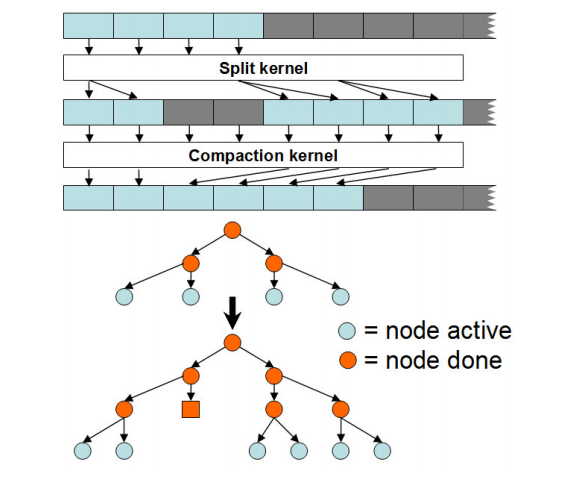
\includegraphics[scale=0.7]{SAH1.png}
\caption{工作队列的构建,通过使用两个工作队列,可以并行运行所有激活的拆分操作。 由于拆分内核可能不会输出新的拆分,因此每次拆分步骤之后会进行压缩操作来删除队列中的空白空间。}
\end{center}
\end{figure}
\item[(2)]{\bm{数据并行处理}} \mbox{}\\
为对象层次结构执行SAH拆分操作包括两个步骤:
\begin{itemize}
\item{通过评估SAH确定最佳分割位置;}
\item{基元的重排序,与Kd-tree等空间分区方法不同,重排序不需要额外的内存。}
\end{itemize}
上述两个步骤都可以通过利用数据并行性和使用常见的并行操作来执行,并且每个拆分操作都在一个核上执行。
\item[(3)]{\bm{细小拆分操作的优化}} \mbox{}\\
针对由于层次结构的顶层初始拆分阶段缺乏并行性以及在最后存在很多的细小拆分导致的算法速度瓶颈问题。
本文中使用每个处理器的本地内存来维护所有的本地工作队列。由于cache非常快,从而较少了内存访问等待时间。除此之外,内核中使用尽可能少的线程来最大化利用向量运算。 分割为“小”的基元的阈值取决于可以将多少几何数据存储到本地存储器中。
\end{itemize}

\subsection{Karras和Apetrei的并行优化}
\subsubsection{基本原理}
2012年Tero Karras在基数树的基础上提出了一种LBVHs的改进算法,从而减少了LBVHs在构建时的耗时\upcite{karras}。
\par Karras在其文中指出传统的构建包围盒和八叉树是基于在空间填充曲面内对原始数据进行排序,该方法的缺点无法并行的进行。该文中方法整体流程如下所示:
\begin{itemize}
\item[(1)]{给每个原始数据根据其质心进行莫顿码赋值;}
\item[(2)]{对莫顿码进行排序;}
\item[(3)]{构建二叉基数树;} \mbox{} \\
传统的构建基数树的方式是一种串行的方式。为了使得构建的过程并行化,Karras为内部节点分配了索引,并且利用一个特定的树布局来建立节点索引和关键值之间的关系,使其能够在不依赖于早期结果的情况下查找其子节点。文中提到的用来帮助实现并行化的二叉基数树示意图如下图所示,树中每个内部节点都被分配了一个介于0-6之间的索引,并与相同索引的叶节点水平对齐。 由每个节点覆盖的键的范围由水平条指示,并且根据键值的第一个比特位的不同,将位置进行区分开来由红色圆圈表示。
\begin{figure}[H]
\begin{center}
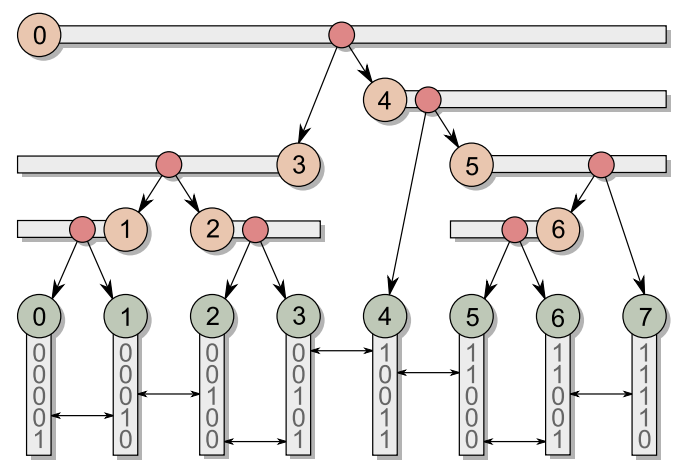
\includegraphics[scale=0.5]{parallel_binary_radix_tree.png}
\caption{并行构建二叉基数树示意图}
\end{center}
\end{figure}
\item[(4)]{给二叉基数树的内部节点赋予包围盒;}
\end{itemize}

\par 2014年Apetrei有在Karras方法上做了进一步改进\upcite{apetrei}。相比于原始方法在排序阶段有了将近50\%的速度提升。Apetrei从两个方面改进了Karras的方法。第一方面是将层次结构和包围盒产生放在同一个cuda的kernel中来完成。与Karras不同的是Apetrei采用的是自下而上的构建顺序,既从每一个键出发,把这些键一层一层的归并到某个簇中,直到顶层节点包含了所有的键。第二方面是将内部索引关系和涵盖的键范围建立步骤相合并,通过跟踪键的范围作为自下而上减少的一部分,并使用它们推导每个步骤的父节点的索引。 每个叶节点都覆盖一个键的范围,每个内部节点合并其子节点的范围。



\section{基于深度控制的优化方案}
\subsection{基本原理}
1983年Hall, Roy A.和Donald P. Greenberg\upcite{Hall}等人提出了一种自适应深度的方法来减少光束的数量。
他们将光线跟踪的分为四个步骤:(1)给物理环境建模;(2)对光线在环境中的传播进行仿真;(3)确定成像平面的密度函数;(4)将离散成像平面密度信息转化为可显示的形式。
\par 传统上,任何采样点的交叉树被构造成预先指定的任意深度以确保能够捕获足够的与产生的图片相关的反射和折射信息。然而对于大多数典型环境,由反射或者透明表面组成的场景占比很少。因此有很大的空间去优化树的的深度。
\par 该文中将交点树中任何节点的贡献值的上界近似为最终采样点的颜色值,通过考虑树种每个节点的强度来使得强度达到最大。第一个节点在树上将贡献100%的最终颜色样本点。子节点的最大贡献值可以通过将代表反射孩子节点设置统一为$I_r$和$F_r$,将传输的孩子节点设置统一为$I_t$和$F_t$,最终算出相关的贡献率。可以对树中任何父节点的子节点重复此过程。 通过乘以近似最大贡献,可以计算子节点对样本点的最大累积贡献。因此,通过建立截止贡献阈值,从而可以在光线跟踪过程中自适应地控制树的深度。


\section{基于层次包围盒(BVH)的改进方法}
我们将对象组包含在分层边界体积集中,并首先测试与边界体积的交集,然后仅在有交叉点的情况下对着体积所包围的对象进行测试。
\par 边界体积应易于测试交叉点,例如球体或盒子(平板)。 最佳边界体积将由底层对象的形状决定。 例如,如果对象是长而薄的,那么球体将主要包围空白空间并且盒子要好得多。 对于分层边界卷,框也更容易。使用这样的分层系统(假设它已经仔细完成)会将交叉点计算时间从对象数量的线性依赖性改变为线性和逻辑关系之间的某种程度。 这是因为,对于一个完美的情况,每个求交测试会将可能性划分为两个,并且我们将具有二叉树类型结构。
\subsection{基本概念}
\subsubsection{BVH}
BVH英文全称Bounding Volume Hierarchies,边界体积层次结构(BVH)已广泛存在用于光线跟踪和碰撞检测。在交互式光线跟踪领域中,基于对象层次结构的方法由于Kd-Tree技术在CPU和GPU上得到了发展而重新获得关注。早期的方法使用简单的更新技术来维护动态数据集并且使用快速构建技术来重建BVH\upcite{LBVH}。

\subsubsection{LBVH}
2009年Lauterbach等人引入了BVH构造算法,该算法基于在场景边界框内运行的填充莫顿曲线对基元进行排序。空间填充曲线长期以来一直用于改进空间算法。可以计算沿着$n$阶莫尔顿曲线的三维点的坐标,也称为其莫顿码,将其坐标离散化为$n$位并交织它们的二进制数,从而获得$3n$位索引。 由于算法将构建层次结构的问题转化为沿曲线排序一组点的问题,Lauterbach等人将其称为线性边界体积层次(LBVH)算法。该方法的构建步骤如下所示:
\begin{figure}[H]
\begin{center}
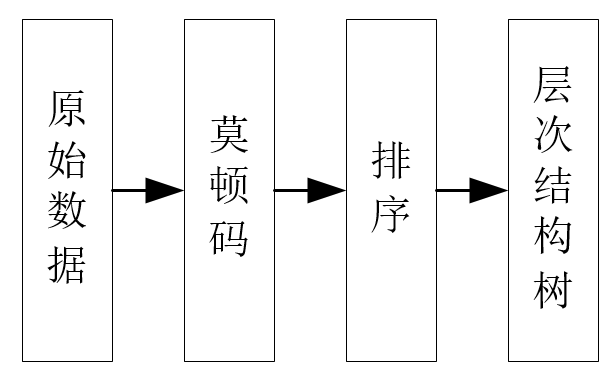
\includegraphics[scale=0.4]{LBVH.png}
\caption{LBVH构建步骤示意图}
\end{center}
\end{figure}

\subsubsection{表面积启发式算法(SAH)}
SAH英文全称Surface Area Heuristic,中文称为表面积启发式算法,表面积启发式算法法基于的理论是复杂度成本分析和概率论,主要用于解决怎样划分轴的问题,可以被应用到适用于多种类型的分层加速结构。


\subsubsection{莫顿码(Morton Code)}
莫顿码可以将多维数据转化为一维数据编码,根据一维编码位数可确定多维数据保留精度,是一种比较常用的压缩编码方法,尤其是作为哈希表的映射算法等,加速了树结构数据的存储和访问速度。莫顿码引入空间填充曲线,它提供了一种稳定的量化矢量的稳定排序方法,这意味着具有相同子序列莫顿码的矢量在空间上是彼此接近。虽然有其他形式的空间填充曲线,但是莫顿码计算的简单性使得它得到了广泛的运用。莫顿码可以通过几次简单的比特交叉操作得到。如下图所示是二维莫顿码的简单示例:
\begin{figure}[H]
\begin{center}
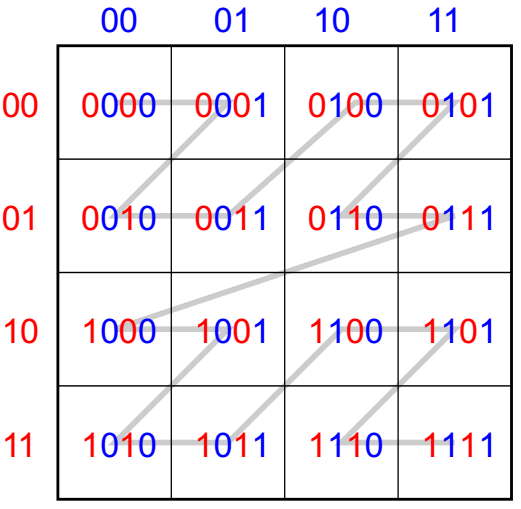
\includegraphics[scale=0.4]{morton-code.png}
\caption{二维4比特莫顿码示意图}
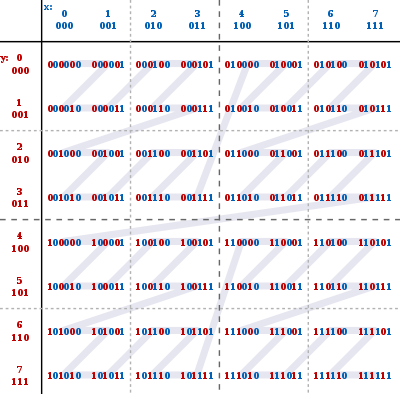
\includegraphics[scale=0.7]{morton-code3.png}
\caption{二维6bit莫顿码示意图}
\end{center}
\end{figure}

\par 莫顿码的一个主要参数是该码的位数。莫顿码的产生步骤如下:
\begin{itemize}
\item[(1)]{\bm{确认量化坐标}}:例如对应三维的莫顿码其量化坐标为$\bm{v}^{*}=\{v_x^{*},v_y^{*},v_z^{*}\}$

\item[(2)]{\bm{交叉操作}}:例如对应的三维莫顿码,假设量化坐标$v_x^{*}=x_7x_6x_5x_4x_3x_2x_1x_0$,$v_y^{*}=y_7y_6y_5y_4y_3y_2y_1y_0$,$v_z^{*}=z_7z_6z_5z_4z_3z_2z_1z_0$,利用交叉操作得到的莫顿码为
$$
m(v^{*})=x_7y_7z_7x_6y_6z_6x_5y_5z_5x_4y_4z_4x_3y_3z_3x_2y_2z_2x_1y_1z_1x_0y_0z_0
$$
\end{itemize}
查表法可用于预先计算某些位范围的代码,然后在运行时通过简单的添加和组合进行组合。

\subsection{Hank Weghorst等人改进方案}
1987年Hank Weghorst等人\upcite{Hank}指出传统的光线跟踪算法是从视角出发反向回到环境中,其具体的步骤如下:
\begin{itemize}
\item[(1)]{首先求解光线与最近表面的交点,之后会得到反射和折射光线;}
\item[(2)]{接下来进一步递归的产生反射折射光线,从而得到所有的相交面;}
\item[(3)]{在递归求解交点的过程中,一个与采样点相对应的由交点构成的树形结构会被建立起来;}
\item[(4)]{最终光照密度通过累加树中每个节点的光密度与贡献值的乘积求得。}
\end{itemize}

该文中从三个角度对光线跟踪算法的进行改进。第一个角度是选择合理的包围盒;第二个角度是对层次结构的建立过程进行改进;第三个角度是利用对象存在的连续性提出了一种可见表面预处理方法。

\subsubsection{包围盒的选取}
该文中指出在包围盒的选取过程中需要考虑的因素有面和基平行、空白投影区域、包围物体的复杂性。空白区域是指包围盒与物体投影区域的差值,如下图所示:
\begin{figure}[H]
\begin{center}
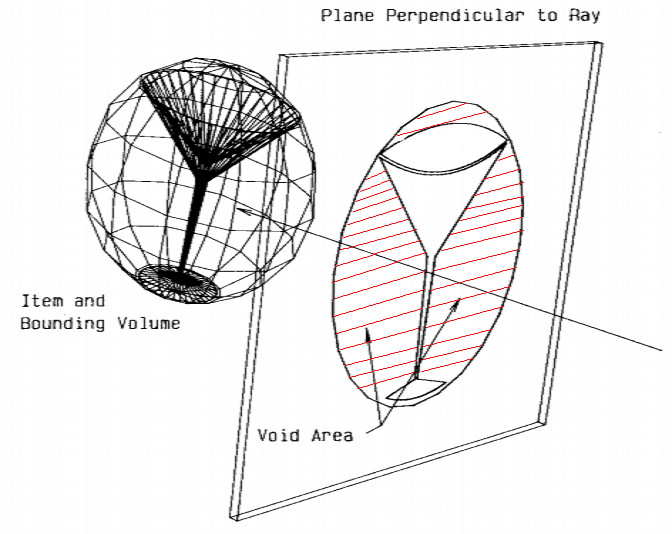
\includegraphics[scale=0.6]{void_area.png}
\caption{投影空白区域示意图(红色阴影线部分)}
\end{center}
\end{figure}
则选取包围盒时,应该使得空白面积最小化。综合上述因素,则总的耗时函数可以表示如下:
$$T=bB+iI$$
其中,$T$为总的耗时,$b$是交点检测中包围盒被检测的次数,$B$单个包围盒检测交点的耗时,$i$物体交点检测的次数,$I$物体交点检测的耗时。
当物体指定是$b$和$I$是一个常值,通过改变包围盒的大小和形状,$B$和$i$可以被改变从而减少整体的耗时。
\par 综合考虑上述因素之后,选取物体的包围盒首先需要确定包围该物体的一个点集,该点集组成的多面体是该物体的凸包,其中最优的凸包顶点集合应该满足的条件是是让多面体与物体的体积之差最小。因此该文中提出了一个包围盒选取的方案,其选取步骤如下所示:
\begin{itemize}
\item[(1)]{给定一组包围盒的候选集,例如球体、长方体、圆柱体;}
\item[(2)]{给包围盒候选集中的所有元素指定一个因子,该因子与交点检测的复杂度相关,例如球的该因子最小,而圆柱体的该因子最大;}
\item[(3)]{包围盒选取的结果为使得选定的元素对应的因子与物体对应的潜在边界形状体积的乘积。}
\end{itemize}
\subsubsection{层次结构的建立改进}
传统方法中,层次结构中引入了组的概念。距离比较相近的物体可以被归并到同一个组,而同一组又可以用一个包围盒来表示。而这个包围组的包围盒相对于物体的包围盒更高一层。
\par 本文中提出为了简化过程,可以将组内只有一个元素的组从层次结构中剔除。这样的简化过程得到的结果依然能够满足用户的要求。

\subsubsection{基于可见表面的预处理方法}
由于可见表面必然与观察者最为接近,该文中借鉴了Z-buffer算法的方法产生Item Buffer,从而对物体的前后顺序得到一种索引列表,随后光线跟踪算法便可以根据该索引列表得到第一个光线交点,从而改进光线跟踪中求交的速度,Weghorst建议使用修改的Z缓冲算法来确定第一次命中。

\subsection{基于HLBVH的方法}
2010年J. Pantaleoni和D. Luebke提出了HLBVH方法\upcite{HLBVH}。HLBVH英文全称Hierarchical Linear Bounding Volume Hierachies。涉及到的主要技术有莫顿码构建线性层次包围盒、表面积启发式算法、hierachy emission algorithm。

\begin{itemize}
\item[(1)]{首先利用莫顿码给场景中的规则化网格进行编码;}
\item[(2)]{将LBVH算法分成两层结构,在第一层中根据$m$位的莫顿曲线将基元排序为$3m$位的网格,在第二层对剩下的3个比特位对基元进行排序;}
\item[(3)]{为每个基元计算和存储30位的莫顿码。}
\item[(4)]{使用层次排放算法,该算法的核会找出其中比较重要的比特位,其步骤如下所示:}
\begin{itemize}
\item{首先,原始数组根据每一个叶子节点在当前输出结构中的位置从概念上将初始数组分割为几个组。}
\item{根据这些组产生一个深度为$p$小树结构,这些小树结构可以在列表中完整描述每个段中的分裂平面。}
\end{itemize}
\end{itemize}


\section{总结}
本文针对渲染中常用的加速技术进行了调研,主要涉及了三个方面的加速方案并行加速方案、基于BVH的加速方案、减少光线个数的方案。如下表所示是对上述多种方案的结果总结:

\begin{table}[H]
\begin{center}
\caption{各种方法的耗时数量级总结}
\begin{tabular}{ccccc}

\toprule  %添加表格头部粗线

方法分类&年代&方法名称(或作者)&耗时数量级\\

\midrule  %添加表格中横线
\multirow{2}*{基于GPU并行方案}&2009年& Lauterbach等人&毫秒级 \\
\cline{2-4}
~&2012年和2014年&Karras和Apetrei&毫秒级\\
\hline
深度控制方案&1983年&Hall等人&分钟级 \\
\hline
\multirow{2}*{基于BVH的优化方案}&1987年&Weghorst等人&小时级 \\
\cline{2-4}
~&2010年&HLBVH(同时使用了GPU并行)&毫秒级\\
\bottomrule %添加表格底部粗线

\end{tabular}
\end{center}
\end{table}

通过上表可以发现,并行方案对于耗时的优化效果较好,并且由于BVH的方案能够与并行方案相结合,因此近年来基于BVH的优化方案研究较多。

\begin{thebibliography}{3}
\bibitem{LBVH} Lauterbach, Christian, et al. "Fast BVH construction on GPUs." Computer Graphics Forum. Vol. 28. No. 2. Oxford, UK: Blackwell Publishing Ltd, 2009.

\bibitem{karras} Karras, Tero. "Maximizing parallelism in the construction of BVHs, octrees, and k-d trees." Proceedings of the Fourth ACM SIGGRAPH/Eurographics conference on High-Performance Graphics. Eurographics Association, 2012.

\bibitem{apetrei} Apetrei, Ciprian. "Fast and simple agglomerative LBVH construction." (2014).


\bibitem{Hall} Hall, Roy A., and Donald P. Greenberg. "A testbed for realistic image synthesis." IEEE Computer Graphics and Applications 3.8 (1983): 10-20.

\bibitem{Hank}Weghorst, Hank, Gary Hooper, and Donald P. Greenberg. "Improved computational methods for ray tracing." ACM Transactions on Graphics (TOG) 3.1 (1984): 52-69.



\bibitem{accelerator3} Woop, Sven, Attila T. Áfra, and Carsten Benthin. "STBVH: a spatial-temporal BVH for efficient multi-segment motion blur." Proceedings of High Performance Graphics. ACM, 2017.

\bibitem{accelerator4} Vinkler, Marek, Jiri Bittner, and Vlastimil Havran. "Extended Morton codes for high performance bounding volume hierarchy construction." Proceedings of High Performance Graphics. ACM, 2017.

\bibitem{cpus1} Havran, Vlastimil, Robert Herzog, and Hans-Peter Seidel. "On the fast construction of spatial hierarchies for ray tracing." Interactive Ray Tracing 2006, IEEE Symposium on. IEEE, 2006.



\bibitem{HLBVH} Pantaleoni, Jacopo, and David Luebke. "HLBVH: hierarchical LBVH construction for real-time ray tracing of dynamic geometry." Proceedings of the Conference on High Performance Graphics. Eurographics Association, 2010.

\bibitem{STBVH} Woop, Sven, Attila T. Áfra, and Carsten Benthin. "STBVH: a spatial-temporal BVH for efficient multi-segment motion blur." Proceedings of High Performance Graphics. ACM, 2017.

\bibitem{accelerator2} Benthin, Carsten, et al. "Improved two-level BVHs using partial re-braiding." Proceedings of High Performance Graphics. ACM, 2017.


\end{thebibliography}
\end{document} 
\end{document}
